\documentclass[10pt,a4paper]{article}
% Compile with XeLaTeX or LuaLaTeX (e.g. tectonic final_report.tex): UTF-8 text with fontspec.
\usepackage[spanish,es-noshorthands,es-tabla]{babel}
\usepackage{amsmath,amssymb}
\usepackage{fontspec}
\usepackage[a4paper,margin=2.2cm]{geometry}
\usepackage{booktabs,tabularx,longtable,multirow,makecell}
\usepackage{graphicx}
\usepackage[table]{xcolor}
\usepackage{enumitem}
\usepackage{caption}
\usepackage[hidelinks]{hyperref}
\usepackage{titlesec}
\usepackage{tcolorbox}

\definecolor{navy}{HTML}{1F3A60}
\titleformat{\section}{\Large\bfseries\color{navy}}{\thesection.}{0.5em}{}
\titleformat{\subsection}{\large\bfseries\color{navy}}{\thesubsection.}{0.5em}{}
\titlespacing*{\section}{0pt}{14pt}{6pt}
\titlespacing*{\subsection}{0pt}{10pt}{4pt}
\captionsetup{font=small,labelfont=bf}
\setlist{itemsep=2pt,topsep=3pt}
\setlength{\parskip}{4pt}
\setlength{\parindent}{0pt}
\setlength{\LTpre}{4pt}
\setlength{\LTpost}{4pt}
\renewcommand{\arraystretch}{1.18}
\graphicspath{{../../results/figures/}{../results/figures/}} % repository / delivery zip

\begin{document}

\hypersetup{pageanchor=false}
\begin{titlepage}
\centering
\vspace*{3cm}
{\color{navy}\rule{\linewidth}{1.2pt}}\\[14pt]
{\Huge\bfseries\color{navy} Cuadrantes de guardias médicas\\[6pt] justos y factibles}\\[14pt]
{\Large Informe final del proyecto}\\[4pt]
{\large Optimización y Simulación · Curso 2026--2027}\\[10pt]
{\color{navy}\rule{\linewidth}{1.2pt}}\\[2cm]
{\large Miguel Troyano Martín\\[2pt] Claudia María López Bombín\\[2pt] María Teresa Sangil Terrés}\\[2cm]
{\large Segunda entrega intermedia, con el formato de la entrega final}\\[4pt]
{\large Noviembre de 2026}
\vfill
{\small Todos los resultados se han obtenido con datos sintéticos generados de forma reproducible.\\ No describen ningún hospital real.}
\end{titlepage}
\hypersetup{pageanchor=true}

\section*{Resumen ejecutivo}
\addcontentsline{toc}{section}{Resumen ejecutivo}

\begin{tcolorbox}[colback=navy!4,colframe=navy,boxrule=0.6pt,arc=2pt,left=8pt,right=8pt,top=6pt,bottom=6pt]
\textbf{Problema.} Cada mes, un servicio hospitalario decide qué residente (MIR) cubre cada guardia cada día. El cuadrante debe cubrir todas las guardias con personal cualificado, cumplir la normativa, respetar vacaciones y peticiones, dejar personal para la planta y repartir con justicia los fines de semana y festivos. Hoy se hace a mano y el Real Decreto 951/2026 cambiará las reglas en septiembre de 2027.

\smallskip
\textbf{Qué hemos hecho.} Un modelo de optimización entera que, en menos de un segundo, construye el mejor cuadrante posible con cuatro prioridades: (1) cumplir todos los requisitos, (2) respetar las peticiones, (3) repartir con justicia los festivos teniendo en cuenta los meses anteriores y (4) evitar guardias en días alternos. Si un mes no se puede cubrir, el modelo no falla: dice qué falta y qué día. Lo hemos aplicado a un servicio sintético de 15 residentes y resuelto más de 500 variantes.

\smallskip
\textbf{Qué hemos aprendido.}
\begin{itemize}[leftmargin=14pt]
  \item \textbf{En un mes normal el modelo lo cubre todo}, respeta todas las peticiones y reduce la desigualdad en festivos de 21,7 a 14,8, pero el servicio no tiene margen: con un residente menos ya quedan guardias sin cubrir.
  \item \textbf{El RD 951/2026 exige unos 10 residentes más} (de 14 a 24 disponibles) si se mantiene la estructura actual de guardias. Hay que decidir ya entre ampliar plantilla y rediseñar las guardias.
  \item \textbf{En agosto y Navidad faltan personas por cómo coinciden las vacaciones}, no por falta de capacidad nominal. Cada guardia de domingo a jueves deja a un residente fuera de la planta al día siguiente, así que cubrir urgencias y mantener la planta compiten 1 a 1: con la plantilla actual se pueden cubrir todas las guardias de agosto si se reduce la actividad ordinaria en unos 2 residentes al día.
  \item \textbf{La equidad necesita memoria}: equilibrar cada mes por separado no corrige un reparto heredado injusto; teniendo en cuenta los meses anteriores, la desigualdad acumulada se reduce mes a mes.
  \item \textbf{Respetar peticiones y evitar días alternos no cuesta cobertura}: sin esos objetivos el cuadrante incumpliría 4 peticiones al mes y tendría hasta 23 patrones «día sí, día no».
\end{itemize}
\end{tcolorbox}

\newpage


\tableofcontents
\newpage

% =====================================================================
\section{Introducción}
\label{sec:intro}

\paragraph{El problema.} En los hospitales públicos españoles cada servicio elabora cada mes su cuadrante de guardias: decide qué residente (MIR) cubre cada tipo de guardia cada día. El cuadrante tiene que cubrir todas las guardias con residentes cualificados y con suficientes residentes mayores, cumplir la normativa laboral (descanso tras la guardia, máximo mensual), respetar vacaciones, rotaciones externas y peticiones de días libres, dejar personal suficiente para la actividad ordinaria del servicio (planta y consultas) y repartir con justicia, a lo largo del año, las guardias más duras: fines de semana y festivos.

\paragraph{Por qué importa.} Normalmente el cuadrante se hace a mano en una hoja de cálculo. Lleva horas cada mes, a menudo se percibe como injusto y no permite responder a preguntas de planificación como \emph{¿cuántos residentes necesita el servicio para cubrir agosto?} La cuestión es además urgente: el \emph{Real Decreto 951/2026} (BOE de 6 de noviembre de 2026), que modifica el RD~1146/2006, limita desde el 1 de septiembre de 2027 la duración de cada guardia de los residentes a 17~horas y el tiempo de guardia a 68~horas al mes. Hoy un residente puede hacer hasta 7 guardias al mes; con la nueva norma serán, en la práctica, cuatro módulos de 17~h. Los servicios tendrán que rehacer sus cuadrantes y, probablemente, sus plantillas.

\paragraph{Qué aporta este trabajo.} Formulamos el problema como un modelo de programación lineal entera mixta con cuatro objetivos jerarquizados, lo implementamos en Python con Gurobi y lo usamos para responder cuatro preguntas de gestión:
\begin{enumerate}[label=\textbf{P\arabic*.}]
  \item ¿Se puede cubrir el mes con la plantilla actual? Si no, ¿qué falta exactamente y cuándo?
  \item ¿Cuántos residentes necesita el servicio en el régimen actual, con acuerdos locales más estrictos y con el RD~951/2026, y en meses difíciles como Navidad o agosto?
  \item ¿Cómo repartir con justicia los fines de semana y festivos a lo largo de varios meses?
  \item ¿Qué cuesta cada objetivo (peticiones, equidad, patrones agotadores) y qué decisiones de gestión esconde el modelo?
\end{enumerate}

Como seguimos sin autorización para usar datos del hospital, todos los resultados se obtienen con \textbf{datos sintéticos} generados de forma reproducible (Sección~\ref{sec:datos}). Describen un servicio verosímil, no un hospital real: lo que interesa es el mecanismo y el orden de magnitud de los efectos, no las cifras exactas.

El informe se organiza así: la Sección~\ref{sec:datos} describe los datos y supuestos; la Sección~\ref{sec:modelo}, el modelo matemático completo; la Sección~\ref{sec:impl}, la implementación; la Sección~\ref{sec:resultados}, los cuadrantes obtenidos; la Sección~\ref{sec:analisis}, el análisis de sensibilidad, y la Sección~\ref{sec:conclusiones}, las conclusiones y recomendaciones. El Anexo~\ref{app:feedback} recoge los cambios hechos a partir de los comentarios a la propuesta.

% =====================================================================
\section{Datos y supuestos}
\label{sec:datos}

\paragraph{Origen de los datos.} Un generador reproducible (\texttt{notebooks/01\_synthetic\_data\_generation.ipynb}, semilla fija por instancia) construye todos los parámetros del modelo a partir de información pública (normativa, calendario de festivos de la Comunidad de Madrid mediante el paquete \texttt{holidays}) y de los supuestos de la Tabla~\ref{tab:supuestos}, que habría que validar con el servicio. El generador comprueba el dominio y la coherencia de cada parámetro; por ejemplo, que la elegibilidad $E_{rdg}$ y la actividad ordinaria $ROT_{rd}$ salgan del mismo calendario de disponibilidad, para que nadie de vacaciones pueda estar de guardia ni contar en planta. Regenerar los datos reproduce byte a byte los ficheros de \texttt{data/synthetic/}.

\begin{table}[ht]
\centering\small
\caption{Supuestos del generador de datos sintéticos.}
\label{tab:supuestos}
\begin{tabularx}{\linewidth}{@{}p{3.1cm}X@{}}
\toprule
Elemento & Supuesto \\
\midrule
Plantilla & 15 residentes, 3 por año de residencia (R1--R5). Mayores: R3 o superior. \\
Tipos de guardia & Urgencias (\texttt{ED}): 2 residentes al día, al menos 1 mayor y como mucho 1 R1. Planta (\texttt{WARD}): 1 residente al día, R2 o superior. En total, 3 plazas al día y 93 en un mes de 31 días. \\
Límites mensuales & Mínimo formativo de 4 guardias, prorrateado por los días disponibles; máximo de 7 (RD 1146/2006). \\
Actividad ordinaria & 9 residentes necesarios cada día laborable ($PL_d = 9$), también en verano. \\
Días duros ($\mathcal{F}$) & Sábados, domingos y festivos de la Comunidad de Madrid. \\
Disponibilidad & Un residente de rotación externa todo el mes, bloques de vacaciones y días sueltos de curso. \\
Peticiones & De 0 a 3 días pedidos libres por residente (la mitad en fin de semana), con prioridad 1 (50\,\%), 2 (35\,\%) o 3 (15\,\%). \\
Histórico & Año de residencia desde junio. Guardias en festivo previas generadas con un sesgo individual, de modo que el reparto heredado está desequilibrado. \\
Mes anterior & 3 residentes de guardia el último día y otros 3 el penúltimo. \\
\bottomrule
\end{tabularx}
\end{table}

\paragraph{Instancias.} Usamos siete meses (Tabla~\ref{tab:instancias}). Enero de 2027 es el mes base. Diciembre de 2026 (tres festivos y seis bloques de vacaciones de 7 días) y agosto de 2027 (ocho residentes con 14 días de vacaciones) son los meses difíciles. Febrero a mayo de 2027 continúan enero y sirven para simular varios meses seguidos (Sección~\ref{sec:equidad}).

\begin{table}[ht]
\centering\small
\caption{Instancias sintéticas. Capacidad nominal: suma de los máximos mensuales $G^{\protect\max}_r$. Déficit estructural en planta: residentes que faltarían en planta aunque nadie hiciera guardias, $\sum_{d \in \mathcal{L}} \protect\max\bigl(0, PL_d - \sum_r ROT_{rd}\bigr)$. En todas las instancias hay 14 residentes disponibles para guardias (el decimoquinto está de rotación externa todo el mes).}
\label{tab:instancias}
\setlength{\tabcolsep}{4pt}
\begin{tabular}{@{}lccccccc@{}}
\toprule
Instancia & Días & \makecell{Días\\ duros $|\mathcal{F}|$} & \makecell{Plazas de\\ guardia} & \makecell{Capacidad\\ nominal} & \makecell{Residentes con\\ vacaciones\\ (días)} & \makecell{Déficit\\ estructural\\ en planta} & Peticiones \\
\midrule
Enero 2027 (base)        & 31 & 12 & 93 & 98 & 2 (10)  & 0 & 17 \\
Diciembre 2026 (Navidad) & 31 & 11 & 93 & 98 & 6 (42)  & 0 & 12 \\
Agosto 2027 (verano)     & 31 &  9 & 93 & 98 & 8 (112) & 7 & 21 \\
Febrero 2027             & 28 &  8 & 84 & 98 & 2 (10)  & 0 & 13 \\
Marzo 2027               & 31 & 11 & 93 & 98 & 2 (10)  & 0 & 26 \\
Abril 2027               & 30 &  8 & 90 & 98 & 2 (10)  & 0 & 34 \\
Mayo 2027                & 31 & 11 & 93 & 98 & 2 (10)  & 0 & 23 \\
\bottomrule
\end{tabular}
\end{table}


\paragraph{Implicaciones de los supuestos.}
\begin{itemize}
  \item \textbf{El servicio va justo.} Hay 93 plazas al mes y una capacidad nominal de $14 \times 7 = 98$ guardias (un residente está fuera todo el mes). Con un margen tan pequeño, cualquier ausencia se nota, lo que hace interesante el análisis de plantilla.
  \item \textbf{Agosto es pesimista.} Mantener $PL_d = 9$ en agosto supone que la actividad ordinaria no se reduce en verano. Con las vacaciones, ya faltan residentes en planta aunque nadie hiciera guardias (déficit estructural de la Tabla~\ref{tab:instancias}). La Sección~\ref{sec:planta} cuantifica cuánto cambia el resultado si se relaja este requisito.
  \item \textbf{El histórico desequilibrado} hace que la equidad con memoria tenga trabajo que hacer; con un histórico perfectamente equilibrado el criterio de equidad apenas cambiaría el cuadrante.
\end{itemize}

\paragraph{Escenarios normativos.} \textbf{Escenario A} (régimen actual, RD 1146/2006): como máximo 7 guardias al mes; quien está de guardia un día laborable trabaja antes la jornada ordinaria de mañana. \textbf{Escenario B} (RD 951/2026, desde septiembre de 2027): guardias de 17~h como máximo, contando la jornada ordinaria si es consecutiva, y 68~h de guardia al mes. Como el servicio aún no ha rediseñado sus tipos de guardia, aproximamos B suponiendo que todas las guardias son módulos de 17~h (Sección~\ref{sec:impl}).

% =====================================================================
\section{Modelo matemático}
\label{sec:modelo}

El modelo decide qué residente cubre cada tipo de guardia cada día del mes. Es un modelo de programación lineal entera mixta (MILP) con cuatro objetivos ordenados por prioridad.

\paragraph{Convención de notación.} Los \textbf{parámetros} (datos de entrada) se escriben en \textbf{mayúsculas} ($N_{dg}$, $E_{rdg}$, $ROT_{rd}$\dots) y las \textbf{variables de decisión} en \textbf{minúsculas} ($x_{rdg}$, $h_{dg}$, $e^{\max}$\dots). Cada símbolo se describe indicando el significado de todos sus subíndices: $r$ es siempre un residente, $d$ un día y $g$ un tipo de guardia. Cada elemento ocupa una línea: primero el símbolo, después su nombre y después lo que modela; en las restricciones, primero el nombre y después la formulación.

\subsection{Conjuntos}

{\small
\begin{longtable}{@{}p{2.6cm}p{3.0cm}p{10.0cm}@{}}
\toprule
Símbolo & Nombre & Qué modela \\
\midrule
\endhead
$r \in \mathcal{R}$ & Residentes & Residentes (MIR) que entran en el cuadrante del servicio. \\
$\mathcal{R}_S \subseteq \mathcal{R}$ & Residentes mayores & Residentes con experiencia suficiente para garantizar la seguridad de una guardia (aquí, R3 o superior). \\
$\mathcal{R}_1 \subseteq \mathcal{R}$ & Residentes de primer año & Residentes R1, cuyo número por guardia está limitado. \\
$d \in \mathcal{D}$ & Días del mes & Días del mes que se planifica, $\mathcal{D} = \{1, \dots, n\}$, donde $n$ es el número de días del mes. \\
$d \in \{-1, 0\}$ & Días del mes anterior & Penúltimo ($d = -1$) y último ($d = 0$) día del mes anterior. Solo aparecen a través de datos, para enlazar el descanso y los patrones con el mes previo. \\
$g \in \mathcal{G}$ & Tipos de guardia & Tipos de guardia del servicio (aquí, urgencias \texttt{ED} y planta \texttt{WARD}). \\
$\mathcal{F} \subseteq \mathcal{D}$ & Días duros & Sábados, domingos y festivos del mes: las guardias más penosas, que deben repartirse con justicia. \\
$\mathcal{L} = \mathcal{D} \setminus \mathcal{F}$ & Días laborables & Días con actividad ordinaria (planta y consultas). \\
$\mathcal{P} \subseteq \mathcal{R} \times \mathcal{D}$ & Peticiones de día libre & Pares $(r, d)$ tales que el residente $r$ ha pedido no tener guardia el día $d$. \\
$\mathcal{R}^F \subseteq \mathcal{R}$ & Residentes comparados en equidad & Residentes con $\Phi_r > 0$ que pueden hacer alguna guardia en un día de $\mathcal{F}$ este mes. Se excluye a quien no puede recibir festivos este mes (p.\,ej., de rotación externa), porque su carga no puede cambiar y fijaría artificialmente el máximo o el mínimo. \\
\bottomrule
\end{longtable}\addtocounter{table}{-1}% uncaptioned longtable: do not consume a table number
}

\subsection{Parámetros}

{\small
\begin{longtable}{@{}p{2.6cm}p{3.0cm}p{10.0cm}@{}}
\toprule
Símbolo & Nombre & Qué modela \\
\midrule
\endhead
$N_{dg} \in \mathbb{Z}_{\ge 0}$ & Personas necesarias & Número de residentes necesarios para cubrir la guardia de tipo $g$ el día $d$. \\
$S_{dg} \in \mathbb{Z}_{\ge 0}$ & Mínimo de mayores & Número mínimo de residentes mayores ($\mathcal{R}_S$) en la guardia de tipo $g$ el día $d$. \\
$U_{dg} \in \mathbb{Z}_{\ge 0}$ & Máximo de R1 & Número máximo de residentes de primer año ($\mathcal{R}_1$) en la guardia de tipo $g$ el día $d$. \\
$E_{rdg} \in \{0, 1\}$ & Elegibilidad y disponibilidad & Vale 1 si el residente $r$ está cualificado para la guardia de tipo $g$ y disponible el día $d$ (no está de vacaciones, rotación externa, curso o baja); 0 en otro caso. \\
$G^{\min}_r \in \mathbb{Z}_{\ge 0}$ & Mínimo mensual & Número mínimo de guardias que el residente $r$ debe hacer en el mes por obligación formativa, prorrateado por los días que $r$ está disponible. \\
$G^{\max}_r \in \mathbb{Z}_{\ge 0}$ & Máximo mensual & Número máximo de guardias que el residente $r$ puede hacer en el mes (7 en el escenario A, o menos con acuerdos locales). \\
$Q_{rd} > 0$ & Prioridad de la petición & Importancia de la petición del residente $r$ de no tener guardia el día $d$, para $(r, d) \in \mathcal{P}$. Valores mayores indican peticiones más importantes (aquí 1, 2 o 3). \\
$H_r \in \mathbb{Z}_{\ge 0}$ & Histórico de festivos & Número de guardias en fin de semana o festivo que el residente $r$ ha hecho en los meses anteriores del periodo de referencia (el año de residencia). \\
$\Phi_r \in [0, 1]$ & Fracción disponible & Fracción del periodo de referencia, desde su inicio hasta el mes actual incluido, en la que el residente $r$ ha estado disponible para hacer guardias. \\
$ROT_{rd} \in \{0, 1\}$ & Actividad ordinaria prevista & Vale 1 si el residente $r$ tiene asignada actividad ordinaria (planta, consultas) en el servicio el día laborable $d$; 0 en otro caso (vacaciones, rotación externa, curso). \\
$PL_d \in \mathbb{Z}_{\ge 0}$ & Personal necesario en planta & Número mínimo de residentes necesarios para la actividad ordinaria el día laborable $d$. \\
$Y_{rd} \in \{0, 1\}$ & Guardias del mes anterior & Para $d \in \{-1, 0\}$, vale 1 si el residente $r$ estuvo de guardia el día $d$ del mes anterior ($d = 0$: último día; $d = -1$: penúltimo). \\
$T_g > 0$ & Duración de la guardia & Duración en horas de la guardia de tipo $g$ (solo escenario B). \\
$C_r \in \{0, 1\}$ & Módulo adicional autorizado & Vale 1 si el residente $r$ tiene autorizado un módulo de guardia adicional ese mes (escenario B: solo por razones formativas y con su consentimiento expreso); 0 en otro caso. Es un dato, no una decisión. \\
\bottomrule
\end{longtable}\addtocounter{table}{-1}% uncaptioned longtable: do not consume a table number
}

\subsection{Variables de decisión}

{\small
\begin{longtable}{@{}p{2.6cm}p{3.0cm}p{10.0cm}@{}}
\toprule
Símbolo & Nombre & Qué modela \\
\midrule
\endhead
$x_{rdg} \in \{0, 1\}$ & Asignación & Vale 1 si el residente $r$ cubre la guardia de tipo $g$ el día $d$; 0 en otro caso. Es la decisión principal: el cuadrante. \\
$h_{dg} \ge 0$ & Plazas sin cubrir & Número de plazas de la guardia de tipo $g$ que quedan sin cubrir el día $d$. \\
$h^{S}_{dg} \ge 0$ & Mayores que faltan & Número de residentes mayores que faltan en la guardia de tipo $g$ el día $d$ para llegar al mínimo $S_{dg}$. \\
$h^{P}_{d} \ge 0$ & Personal que falta en planta & Número de residentes que faltan para la actividad ordinaria el día laborable $d$. \\
$h^{G}_{r} \ge 0$ & Guardias por debajo del mínimo & Número de guardias que le faltan al residente $r$ para llegar a su mínimo formativo $G^{\min}_r$. \\
$v_{rd} \ge 0$ & Patrón «día sí, día no» & Vale 1 cuando el residente $r$ está de guardia el día $d$ y también el día $d+2$ (guardia, libre, guardia); 0 en otro caso. \\
$e^{\max}$ & Carga máxima de festivos & Mayor carga normalizada de guardias en fin de semana o festivo entre los residentes de $\mathcal{R}^F$. \\
$e^{\min}$ & Carga mínima de festivos & Menor carga normalizada de guardias en fin de semana o festivo entre los residentes de $\mathcal{R}^F$. \\
\bottomrule
\end{longtable}\addtocounter{table}{-1}% uncaptioned longtable: do not consume a table number
}

\paragraph{Expresión auxiliar.} Para escribir las restricciones de forma compacta usamos
\[
y_{rd} = \sum_{g \in \mathcal{G}} x_{rdg} \quad (d \in \mathcal{D}), \qquad y_{rd} = Y_{rd} \quad (d \in \{-1, 0\}).
\]
$y_{rd}$ no es una variable nueva sino una expresión lineal: vale 1 si el residente $r$ está de guardia (de cualquier tipo) el día $d$ y 0 si no. Para los dos últimos días del mes anterior es un dato.

Las variables de déficit $h_{dg}, h^{S}_{dg}, h^{P}_{d}, h^{G}_{r}$ y $v_{rd}$ se declaran continuas. Como los requisitos $N_{dg}$, $S_{dg}$, $PL_d$ y $G^{\min}_r$ son enteros y $x_{rdg}$ es binaria, en el óptimo toman valores enteros.

\subsection{Función objetivo}

Los cuatro objetivos se optimizan en orden estricto de prioridad (optimización lexicográfica):
\[
\operatorname{lex\,min}\; \bigl(f_1,\; f_2,\; f_3,\; f_4\bigr).
\]
Primero se minimiza $f_1$; después, $f_2$ entre todos los cuadrantes con $f_1$ óptimo; después, $f_3$ entre los que además tienen $f_2$ óptimo, y por último $f_4$.

{\small
\begin{longtable}{@{}p{6.0cm}p{2.4cm}p{7.2cm}@{}}
\toprule
Símbolo & Nombre & Qué modela \\
\midrule
\endhead
$\displaystyle f_1 = \sum_{d \in \mathcal{D}} \sum_{g \in \mathcal{G}} \bigl(h_{dg} + h^{S}_{dg}\bigr) + \sum_{d \in \mathcal{L}} h^{P}_{d} + \sum_{r \in \mathcal{R}} h^{G}_{r}$ & Requisitos incumplidos & Número total de personas que faltan: plazas de guardia sin cubrir, mayores que faltan, residentes que faltan en planta y guardias por debajo del mínimo formativo. Vale 0 si el mes se puede cubrir por completo; si es positivo, el cuadrante dice exactamente qué requisito falla y qué día. Sumar los cuatro déficits con el mismo peso (una persona que falta = 1) es un supuesto de gestión que analizamos en la Sección~\ref{sec:planta}. \\[4pt]
$\displaystyle f_2 = \sum_{(r, d) \in \mathcal{P}} Q_{rd}\, y_{rd}$ & Peticiones incumplidas & Suma de las prioridades de las peticiones incumplidas. Si el residente $r$ pidió libre el día $d$ y aun así tiene guardia ese día, $y_{rd} = 1$ y se suma la prioridad $Q_{rd}$; si la petición se respeta, $y_{rd} = 0$ y no cuesta nada. \\[4pt]
$f_3 = e^{\max} - e^{\min}$ & Equidad & Diferencia entre el residente más cargado y el menos cargado en guardias de fin de semana o festivo, acumuladas en el periodo de referencia y normalizadas por disponibilidad. \\[4pt]
$\displaystyle f_4 = \sum_{r \in \mathcal{R}} \sum_{d = -1}^{n-2} v_{rd}$ & Patrones agotadores & Número de patrones «guardia, libre, guardia», incluidos los que empiezan en el mes anterior. \\
\bottomrule
\end{longtable}\addtocounter{table}{-1}% uncaptioned longtable: do not consume a table number
}

\paragraph{Por qué lexicográfico y no una suma ponderada.} Una suma $W^1 f_1 + W^2 f_2 + W^3 f_3 + W^4 f_4$ solo reproduce una prioridad estricta si cada peso supera el mayor valor posible de todos los términos de menor prioridad juntos. Eso exige pesos de varios órdenes de magnitud, que dan problemas numéricos: la tolerancia del solver puede dejar sin optimizar los términos de menor prioridad. Gurobi resuelve el problema lexicográfico de forma nativa (optimización multiobjetivo jerárquica), así que las prioridades se cumplen exactamente. La Sección~\ref{sec:objetivos} muestra que la suma ponderada da, de hecho, cuadrantes distintos.

\subsection{Restricciones}

\newcommand{\restr}[2]{\par\smallskip\noindent\textbf{(#1) #2.}\par\nopagebreak}

\restr{1}{Cobertura de cada guardia}
\[
\sum_{r \in \mathcal{R}} x_{rdg} + h_{dg} = N_{dg} \qquad \forall d \in \mathcal{D},\; g \in \mathcal{G}
\]
Los residentes asignados a la guardia de tipo $g$ el día $d$, más las plazas que quedan sin cubrir, igualan a las personas necesarias. Nunca se asignan más residentes de los necesarios. Si faltan residentes, $h_{dg}$ dice cuántas plazas quedan vacías en lugar de que el modelo sea infactible.

\restr{2a}{Presencia de residentes mayores}
\[
\sum_{r \in \mathcal{R}_S} x_{rdg} + h^{S}_{dg} \ge S_{dg} \qquad \forall d \in \mathcal{D},\; g \in \mathcal{G}
\]
Cada guardia debe tener al menos $S_{dg}$ residentes mayores, para que haya alguien con experiencia. Si no hay suficientes mayores disponibles, $h^{S}_{dg}$ cuenta cuántos faltan.

\restr{2b}{Límite de residentes de primer año}
\[
\sum_{r \in \mathcal{R}_1} x_{rdg} \le U_{dg} \qquad \forall d \in \mathcal{D},\; g \in \mathcal{G}
\]
Como mucho $U_{dg}$ residentes de primer año en la guardia de tipo $g$ el día $d$, para no concentrar a los menos experimentados.

\restr{3a}{Elegibilidad y disponibilidad}
\[
x_{rdg} \le E_{rdg} \qquad \forall r \in \mathcal{R},\; d \in \mathcal{D},\; g \in \mathcal{G}
\]
Un residente solo puede cubrir los tipos de guardia para los que está cualificado y solo los días en que está disponible. En la implementación, $x_{rdg}$ solo se crea cuando $E_{rdg} = 1$.

\restr{3b}{Como máximo una guardia al día}
\[
y_{rd} \le 1 \qquad \forall r \in \mathcal{R},\; d \in \mathcal{D}
\]
Un residente no puede cubrir dos tipos de guardia el mismo día.

\restr{4}{Descanso tras la guardia}
\[
y_{rd} + y_{r,d+1} \le 1 \qquad \forall r \in \mathcal{R},\; d \in \{0, 1, \dots, n-1\}
\]
Nadie hace guardia dos días seguidos: tras una guardia hay descanso obligatorio. Para $d = 0$ la restricción es $Y_{r0} + y_{r1} \le 1$, es decir, quien estuvo de guardia el último día del mes anterior no puede tener guardia el día 1.

\restr{5}{Evitar guardias en días alternos (restricción blanda)}
\[
y_{rd} + y_{r,d+2} \le 1 + v_{rd} \qquad \forall r \in \mathcal{R},\; d \in \{-1, 0, \dots, n-2\}
\]
Si el residente $r$ tiene guardia los días $d$ y $d+2$ (y, por (4), libra el $d+1$), el lado izquierdo vale 2 y obliga a $v_{rd} = 1$, que se penaliza en $f_4$. No se prohíbe porque a veces es inevitable, pero es un patrón agotador que el modelo evita si puede. Para $d \in \{-1, 0\}$ el patrón cruza el cambio de mes.

\restr{6a}{Mínimo mensual (obligación formativa)}
\[
\sum_{d \in \mathcal{D}} y_{rd} + h^{G}_{r} \ge G^{\min}_r \qquad \forall r \in \mathcal{R}
\]
Las guardias forman parte de la formación del residente: cada uno debe hacer al menos $G^{\min}_r$. Si no es posible, $h^{G}_{r}$ dice cuántas le faltan.

\restr{6b}{Máximo mensual}
\[
\sum_{d \in \mathcal{D}} y_{rd} \le G^{\max}_r \qquad \forall r \in \mathcal{R}
\]
Límite legal (o del acuerdo local) de guardias al mes de cada residente.

\restr{7}{Peticiones de días libres: no requieren restricción}
\par\noindent Se tratan íntegramente en el objetivo $f_2$. Para $(r, d) \in \mathcal{P}$, $y_{rd} = 1$ significa que el residente $r$ tiene guardia un día que pidió libre, es decir, \emph{esa guardia es el incumplimiento de la petición}, y $f_2$ suma su prioridad $Q_{rd}$. En la propuesta usábamos además una variable $s_{rd}$ con $y_{rd} \le s_{rd}$; como $s_{rd}$ se minimiza, en todo óptimo $s_{rd} = y_{rd}$, así que era redundante y la hemos eliminado. Mantenemos la numeración para que sea comparable con la propuesta.

\restr{8}{Reparto justo de fines de semana y festivos (con memoria)}
\[
e^{\min} \le \frac{H_r + \sum_{d \in \mathcal{F}} y_{rd}}{\Phi_r} \le e^{\max} \qquad \forall r \in \mathcal{R}^F
\]
El numerador cuenta las guardias en fin de semana o festivo del residente $r$ en todo el periodo de referencia: las de meses anteriores ($H_r$) más las que se le asignan este mes. Dividir por $\Phi_r$, la fracción del mismo periodo en la que $r$ ha estado disponible, hace comparables a residentes con distinta disponibilidad: quien ha estado disponible la mitad del tiempo debería cargar con la mitad. Como $\Phi_r$ es un dato, la restricción es lineal. $e^{\max}$ y $e^{\min}$ acotan la carga de todos, y $f_3 = e^{\max} - e^{\min}$ mide la diferencia entre el más y el menos cargado. La memoria ($H_r$) permite compensar a lo largo de los meses lo que un solo mes no puede equilibrar.

\restr{9}{Personal suficiente para la actividad ordinaria}
\begin{align*}
&\text{Escenario A:} && \sum_{r \in \mathcal{R}} ROT_{rd}\,\bigl(1 - y_{r,d-1}\bigr) + h^{P}_{d} \ge PL_d \qquad \forall d \in \mathcal{L}\\
&\text{Escenario B:} && \sum_{r \in \mathcal{R}} ROT_{rd}\,\bigl(1 - y_{r,d-1} - y_{rd}\bigr) + h^{P}_{d} \ge PL_d \qquad \forall d \in \mathcal{L}
\end{align*}
El lado izquierdo cuenta cuántos residentes están realmente en el servicio el día $d$ para la planta y las consultas:
\begin{itemize}
  \item $ROT_{rd} = 1$ selecciona a los residentes que ese día tienen actividad ordinaria prevista (no están de vacaciones, rotación externa ni curso).
  \item El factor $(1 - y_{r,d-1})$ resta a los \emph{salientes de guardia}. Una guardia empieza un día y termina a la mañana siguiente; quien estuvo de guardia el día anterior ($y_{r,d-1} = 1$) sale de guardia por la mañana y se va a descansar, así que no trabaja en planta el día $d$ y no cuenta. Por ejemplo, si un residente hace guardia el lunes, el martes es saliente: está en el hospital hasta las 8:00 pero ese martes no cuenta para la planta. Para $d = 1$ el día anterior es el último del mes anterior, dado por $Y_{r0}$.
  \item En el escenario A, quien está de guardia el día $d$ trabaja primero su jornada de mañana y luego empieza la guardia, así que sí cuenta. En el escenario B la jornada ordinaria y la guardia consecutivas no pueden superar 17~h, así que quien está de guardia el día $d$ no hace la jornada de mañana y tampoco cuenta: de ahí el término $-y_{rd}$.
\end{itemize}
Por (4), $y_{r,d-1} + y_{rd} \le 1$, así que el factor vale siempre 0 o 1. Si hay menos de $PL_d$ residentes presentes, $h^{P}_{d}$ dice cuántos faltan. Esta restricción liga el cuadrante de guardias con el funcionamiento diario del servicio: cada guardia en víspera de día laborable cuesta un residente en planta al día siguiente.

\restr{10}{Horas de guardia al mes (solo escenario B)}
\[
\sum_{d \in \mathcal{D}} \sum_{g \in \mathcal{G}} T_g\, x_{rdg} \le 68 + 17\, C_r \qquad \forall r \in \mathcal{R}
\]
Como máximo 68~h de guardia al mes (cuatro módulos de 17~h), más 17~h si el residente tiene autorizado un módulo adicional. $C_r$ es un dato y no una decisión: el módulo adicional solo se justifica por razones formativas y con consentimiento, así que el modelo no puede usarlo para tapar huecos.

\subsection{Garantía de factibilidad}

El modelo siempre tiene solución: $x_{rdg} = 0$ para todo $r, d, g$, con cada déficit igual a su requisito ($h_{dg} = N_{dg}$, $h^{S}_{dg} = S_{dg}$, $h^{P}_{d} = PL_d$, $h^{G}_{r} = G^{\min}_r$), $v_{rd} = 0$ y $e^{\max}$, $e^{\min}$ iguales al máximo y al mínimo de $H_r / \Phi_r$, cumple todas las restricciones. Todo requisito que puede fallar se mide con una variable de déficit en lugar de imponerse como restricción dura. Por eso, en un mes que no se puede cubrir, el modelo no responde «infactible» sino que dice exactamente qué falta y cuándo; un estado «infactible» solo puede indicar un error en los datos.

% =====================================================================
\section{Implementación y reproducibilidad}
\label{sec:impl}

\paragraph{Código.} El modelo está implementado en Python con \texttt{gurobipy} y organizado en tres notebooks:
\begin{itemize}
  \item \texttt{01\_synthetic\_data\_generation.ipynb}: genera y valida las siete instancias (\texttt{data/synthetic/}).
  \item \texttt{02\_baseline\_model.ipynb}: construye el modelo (una función por restricción, precedida de su ecuación), lo resuelve, valida el cuadrante y calcula los indicadores.
  \item \texttt{03\_analysis.ipynb}: reproduce todos los resultados, tablas y figuras de este informe reutilizando el modelo del notebook 02.
\end{itemize}

\paragraph{Decisiones de implementación.}
\begin{itemize}
  \item $x_{rdg}$ solo se crea donde $E_{rdg} = 1$, lo que implementa (3a) sin restricciones explícitas y reduce el tamaño del modelo.
  \item El objetivo lexicográfico usa la optimización multiobjetivo jerárquica de Gurobi (\texttt{setObjectiveN}) con prioridades decrecientes, sin degradación permitida y con cada nivel resuelto hasta optimalidad probada (\texttt{MIPGap} = 0).
  \item Tras resolver, una función independiente de Gurobi comprueba sobre el cuadrante todas las restricciones duras, y todos los indicadores se calculan a partir de $x$, no de las variables de holgura (que solo están ajustadas en el nivel en que se penalizan). En todos los experimentos de este informe (más de 500 resoluciones) la validación no detectó ninguna violación.
  \item \textbf{Aproximación del escenario B.} Sin el rediseño de las guardias del servicio no conocemos las duraciones $T_g$. Suponemos que todas las guardias son módulos de 17~h, de modo que (10) equivale a un máximo de $4 + C_r$ guardias al mes con $C_r = 0$, y usamos la versión B de (9). Como las guardias de 24~h de fin de semana tendrán que partirse, esta aproximación probablemente subestima las necesidades de B.
\end{itemize}

\paragraph{Tamaño y tiempo de resolución.} Para un mes de 31 días el modelo tiene unas 1\,350 variables (unas 750 binarias) y 1\,400 restricciones, y se resuelve en menos de un segundo en un portátil (Tabla~\ref{tab:base}). La licencia de Gurobi incluida con \texttt{pip} limita el modelo a 2\,000 variables y restricciones: basta para los meses base, pero los experimentos con plantillas ampliadas necesitan la licencia académica.

\paragraph{Reproducibilidad.} Los resultados se reproducen instalando \texttt{requirements.txt}, instalando una licencia académica de Gurobi y ejecutando los notebooks 01, 02 y 03 en orden (instrucciones en el \texttt{README.md} de la entrega). Las tablas de resultados se guardan en \texttt{results/tables/} y las figuras en \texttt{results/figures/}. Los indicadores que el modelo optimiza ($f_1$ a $f_4$) son únicos, pero puede haber varios cuadrantes óptimos; indicadores que no se optimizan, como el rango de guardias por residente, pueden variar ligeramente entre versiones de Gurobi.

% =====================================================================
\section{Resultados}
\label{sec:resultados}

Esta sección presenta los cuadrantes que recomienda el modelo para los tres meses de referencia. La Sección~\ref{sec:analisis} analiza cómo cambian al variar los supuestos.

\begin{table}[ht]
\centering\small
\caption{Resultados de los tres meses de referencia (datos sintéticos). Todos los indicadores se calculan a partir del cuadrante $x$. Rango de carga de festivos: $e^{\protect\max} - e^{\protect\min}$ antes y después del mes.}
\label{tab:base}
\setlength{\tabcolsep}{5pt}
\begin{tabular}{@{}lcccccc@{}}
\toprule
 & \multicolumn{2}{c}{Enero 2027} & \multicolumn{2}{c}{Diciembre 2026} & \multicolumn{2}{c}{Agosto 2027} \\
\cmidrule(lr){2-3}\cmidrule(lr){4-5}\cmidrule(lr){6-7}
Escenario & A & B & A & B & A & B \\
\midrule
Plazas de guardia sin cubrir ($h$)            & \textbf{0} & 37 & 5 & 37 & 24 & 47 \\
Mayores que faltan ($h^S$)                    & 0 & 0 & 0 & 2 & 0 & 4 \\
Residentes que faltan en planta ($h^P$)       & 0 & 0 & 1 & 0 & 15 & 19 \\
Guardias por debajo del mínimo ($h^G$)        & 0 & 0 & 0 & 0 & 0 & 0 \\
\textbf{Requisitos incumplidos $f_1$}         & \textbf{0} & \textbf{37} & \textbf{6} & \textbf{39} & \textbf{39} & \textbf{70} \\
Peticiones incumplidas / total                & 0/17 & 0/17 & 0/12 & 0/12 & 0/21 & 0/21 \\
Rango de carga de festivos antes del mes      & 21,7 & 21,7 & 27,5 & 27,5 & 10,3 & 10,3 \\
Rango de carga de festivos después ($f_3$)    & 14,8 & 17,1 & 23,1 & 23,1 & 9,8 & 9,8 \\
Patrones «día sí, día no» ($f_4$)             & 1 & 0 & 0 & 0 & 0 & 0 \\
Guardias por residente (mín.--máx.)           & 5--7 & 4--4 & 4--7 & 4--4 & 2--7 & 2--4 \\
Mín. de residentes en planta (día laborable)  & 9 & 9 & 8 & 9 & 6 & 6 \\
Tiempo de resolución (s)                      & 0,3 & 0,4 & 0,3 & 0,3 & 0,3 & 0,3 \\
\bottomrule
\end{tabular}
\end{table}

\subsection{Mes base: enero de 2027}

En el régimen actual (escenario A) el modelo encuentra un cuadrante que \textbf{cumple todos los requisitos} (Tabla~\ref{tab:base} y Figura~\ref{fig:roster}): cubre las 93 plazas con al menos un residente mayor en cada guardia de urgencias, nunca deja menos de 9 residentes en planta, respeta las 17 peticiones de días libres y solo deja un patrón «guardia, libre, guardia». Cada residente hace entre 5 y 7 guardias. El modelo tiene 1\,352 variables (758 binarias) y 1\,393 restricciones y se resuelve en menos de medio segundo, frente a las horas que lleva hacerlo a mano.

\begin{figure}[ht]
\centering
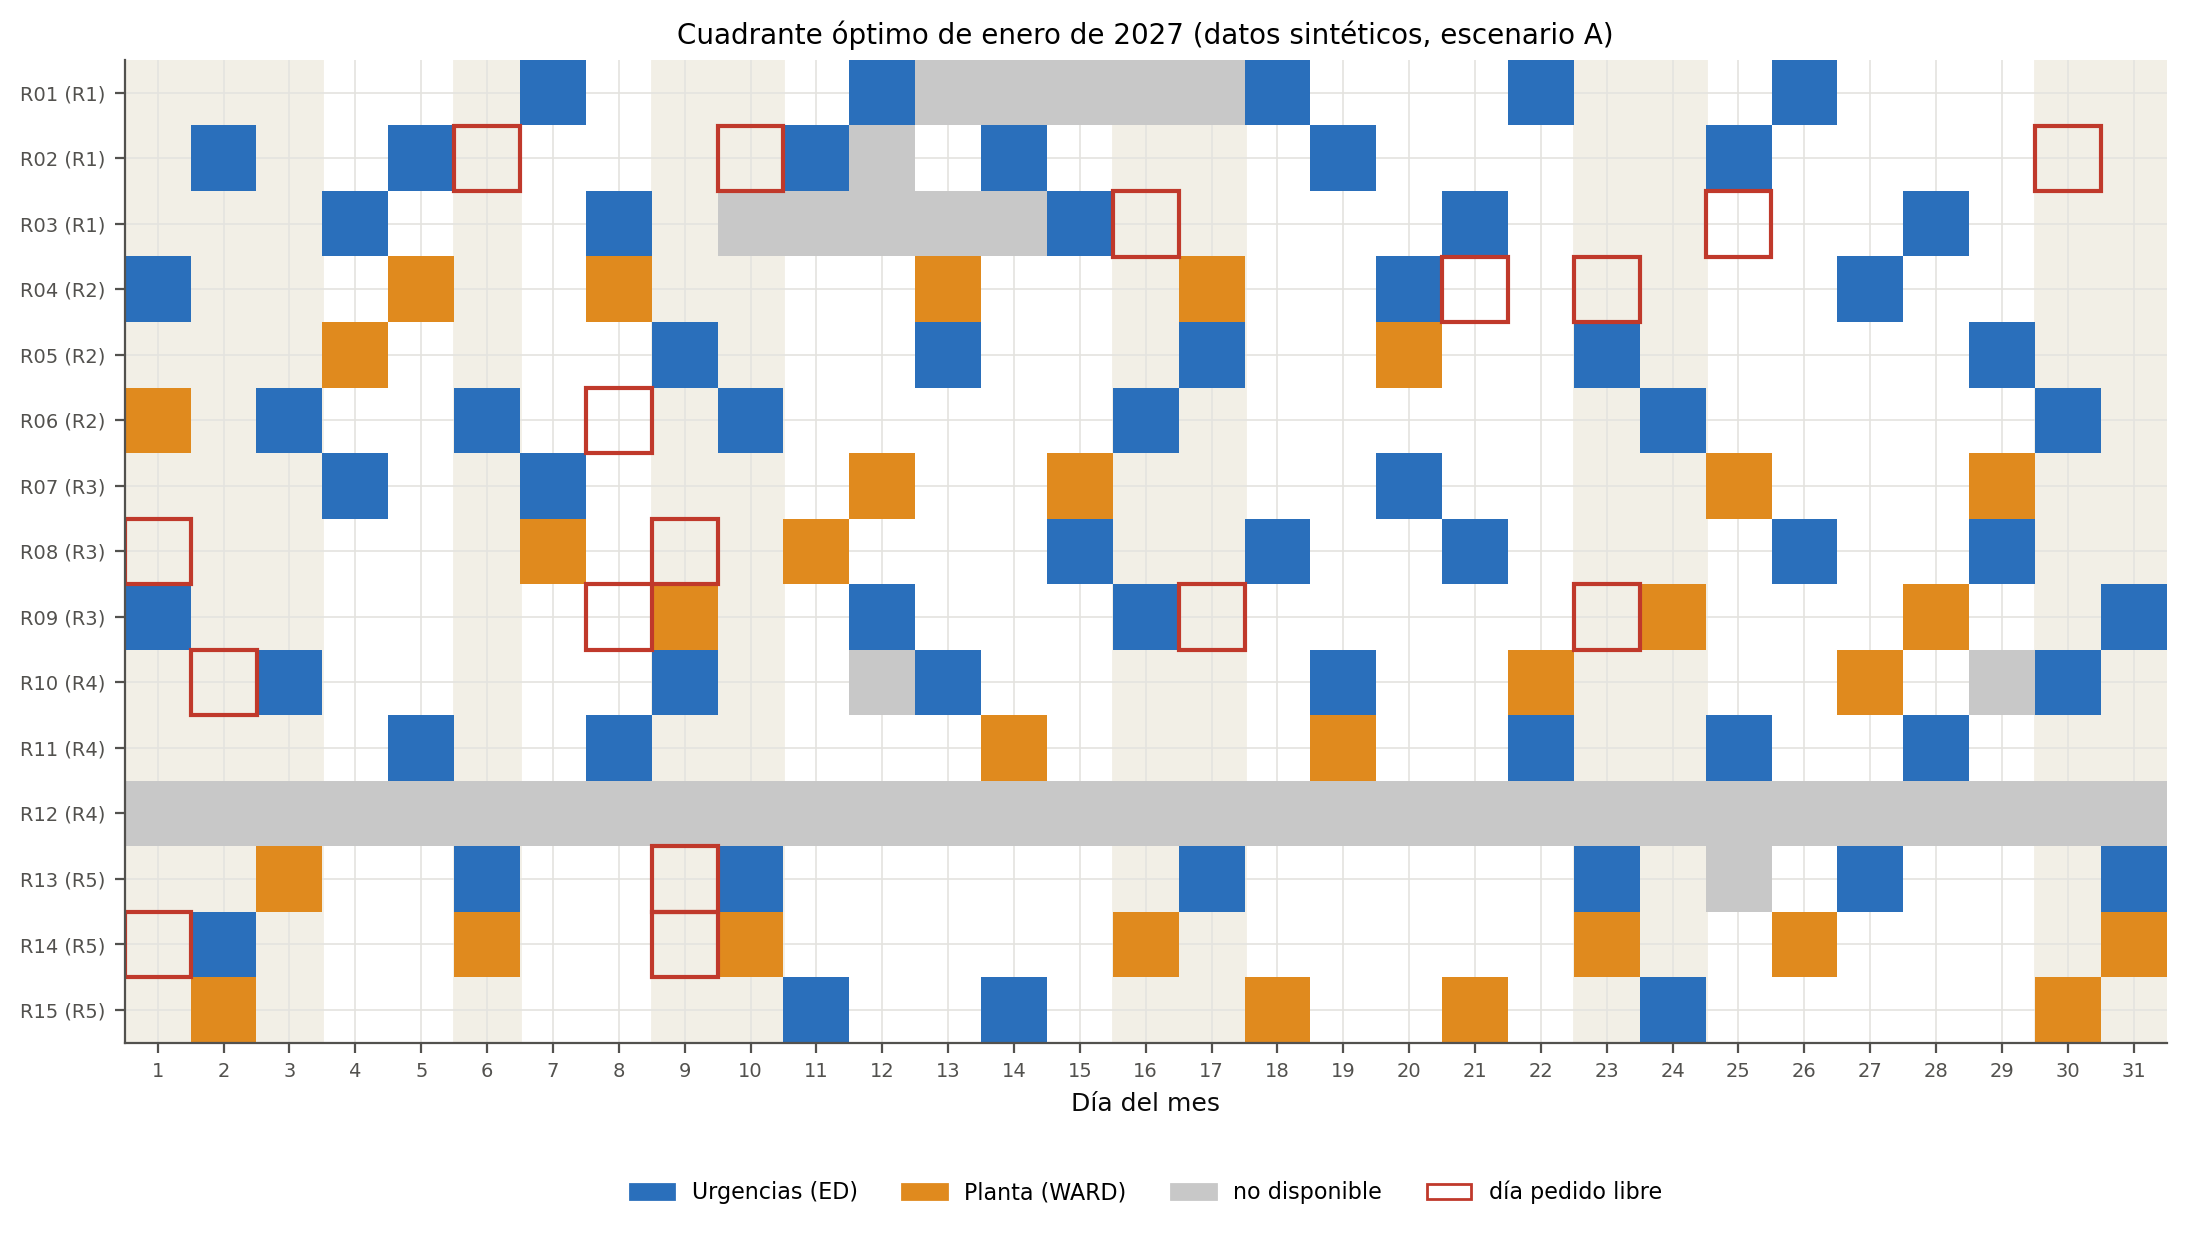
\includegraphics[width=\linewidth]{final_roster_jan2027.png}
\caption{Cuadrante óptimo de enero de 2027 (escenario A). Cada fila es un residente (entre paréntesis, su año de residencia) y cada columna un día. Azul: guardia de urgencias; naranja: guardia de planta; gris: no disponible (vacaciones, rotación externa o curso); recuadro rojo: día pedido libre; columnas sombreadas: fines de semana y festivos.}
\label{fig:roster}
\end{figure}

\paragraph{Equidad.} El modelo asigna los fines de semana y festivos de enero a quienes llevaban menos carga acumulada (Figura~\ref{fig:fairness}): la diferencia entre el residente más cargado y el menos cargado baja de 21,7 a 14,8 guardias normalizadas. No baja más porque el residente más cargado (R07) ya acumula 32 guardias normalizadas: aunque no haga ningún festivo en enero, a los menos cargados no les da tiempo a alcanzarle en un solo mes. Esto es lo que motiva el análisis de varios meses seguidos de la Sección~\ref{sec:equidad}.

\begin{figure}[ht]
\centering
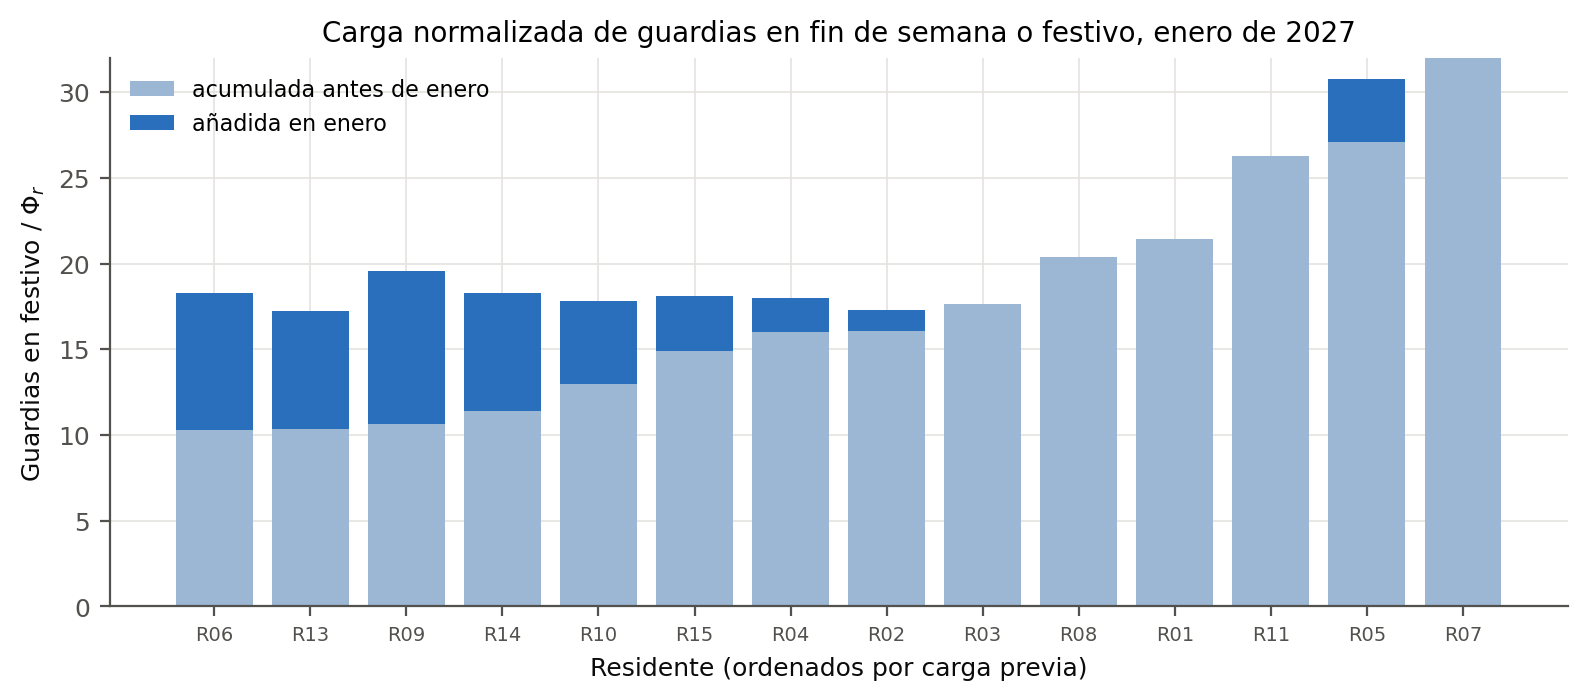
\includegraphics[width=0.78\linewidth]{final_fairness_jan2027.png}
\caption{Carga normalizada de guardias en fin de semana o festivo, $(H_r + \sum_{d \in \mathcal{F}} y_{rd}) / \Phi_r$: acumulada antes de enero (azul claro) y añadida en enero (azul oscuro). Los residentes están ordenados por su carga previa.}
\label{fig:fairness}
\end{figure}

\subsection{Meses difíciles y régimen de 2027}

\paragraph{Diciembre.} Aunque la capacidad nominal es la misma que en enero (98 guardias para 93 plazas), quedan 5 plazas sin cubrir y falta un residente en planta un día. Las vacaciones de Navidad se concentran en las mismas semanas y, con la regla de descanso, quienes quedan no pueden hacer guardias suficientes en esos días: la capacidad real es menor que la nominal.

\paragraph{Agosto.} Con ocho residentes de vacaciones dos semanas, quedan 24 plazas sin cubrir y faltan 15 residentes-día en planta; 7 de esos 15 faltarían aunque nadie hiciera guardias (déficit estructural). Los huecos se concentran en las tres primeras semanas, cuando hay entre 6 y 11 residentes disponibles (frente a 13 o 14 al final del mes), y caen siempre en guardias de domingo a jueves, nunca en viernes ni sábado. La razón es la restricción (9): quien hace guardia un viernes o un sábado sale de guardia en fin de semana y no resta personal de planta, mientras que una guardia de domingo a jueves deja un saliente al día siguiente en una planta que ya va corta. El modelo deja sin cubrir justo las guardias que más cuestan a la actividad ordinaria. La Sección~\ref{sec:planta} analiza este intercambio.

\paragraph{Escenario B (RD 951/2026).} Con un máximo de cuatro guardias de 17~h por residente, los 14 residentes disponibles solo pueden cubrir $14 \times 4 = 56$ de las 93 plazas: quedan 37 sin cubrir en enero y diciembre, y en agosto el déficit total llega a 70 personas. Con la plantilla actual el régimen de 2027 no es viable.

% =====================================================================
\section{Análisis de los resultados}
\label{sec:analisis}

Un único cuadrante óptimo responde a la pregunta P1. Para las preguntas de planificación (P2 a P4) resolvemos el modelo más de 500 veces cambiando la plantilla, el límite mensual, el requisito de planta, la prioridad de los objetivos y la forma de medir la equidad. Cada experimento cambia un único elemento respecto al caso base; todos los cuadrantes se validan de forma independiente.

\subsection{¿Cuántos residentes necesita el servicio?}
\label{sec:plantilla}

Para cada mes y régimen normativo quitamos de 1 a 4 residentes (cinco sorteos aleatorios para cada número) o añadimos de 1 a 12 residentes sintéticos totalmente disponibles. Además del régimen actual (A, 7 guardias) y del RD 951/2026 (B), estudiamos dos acuerdos locales más estrictos que el máximo legal (6 y 5 guardias al mes). La Figura~\ref{fig:plantilla} muestra los requisitos incumplidos $f_1$ y la Tabla~\ref{tab:plantilla} la plantilla mínima.

\begin{figure}[ht]
\centering
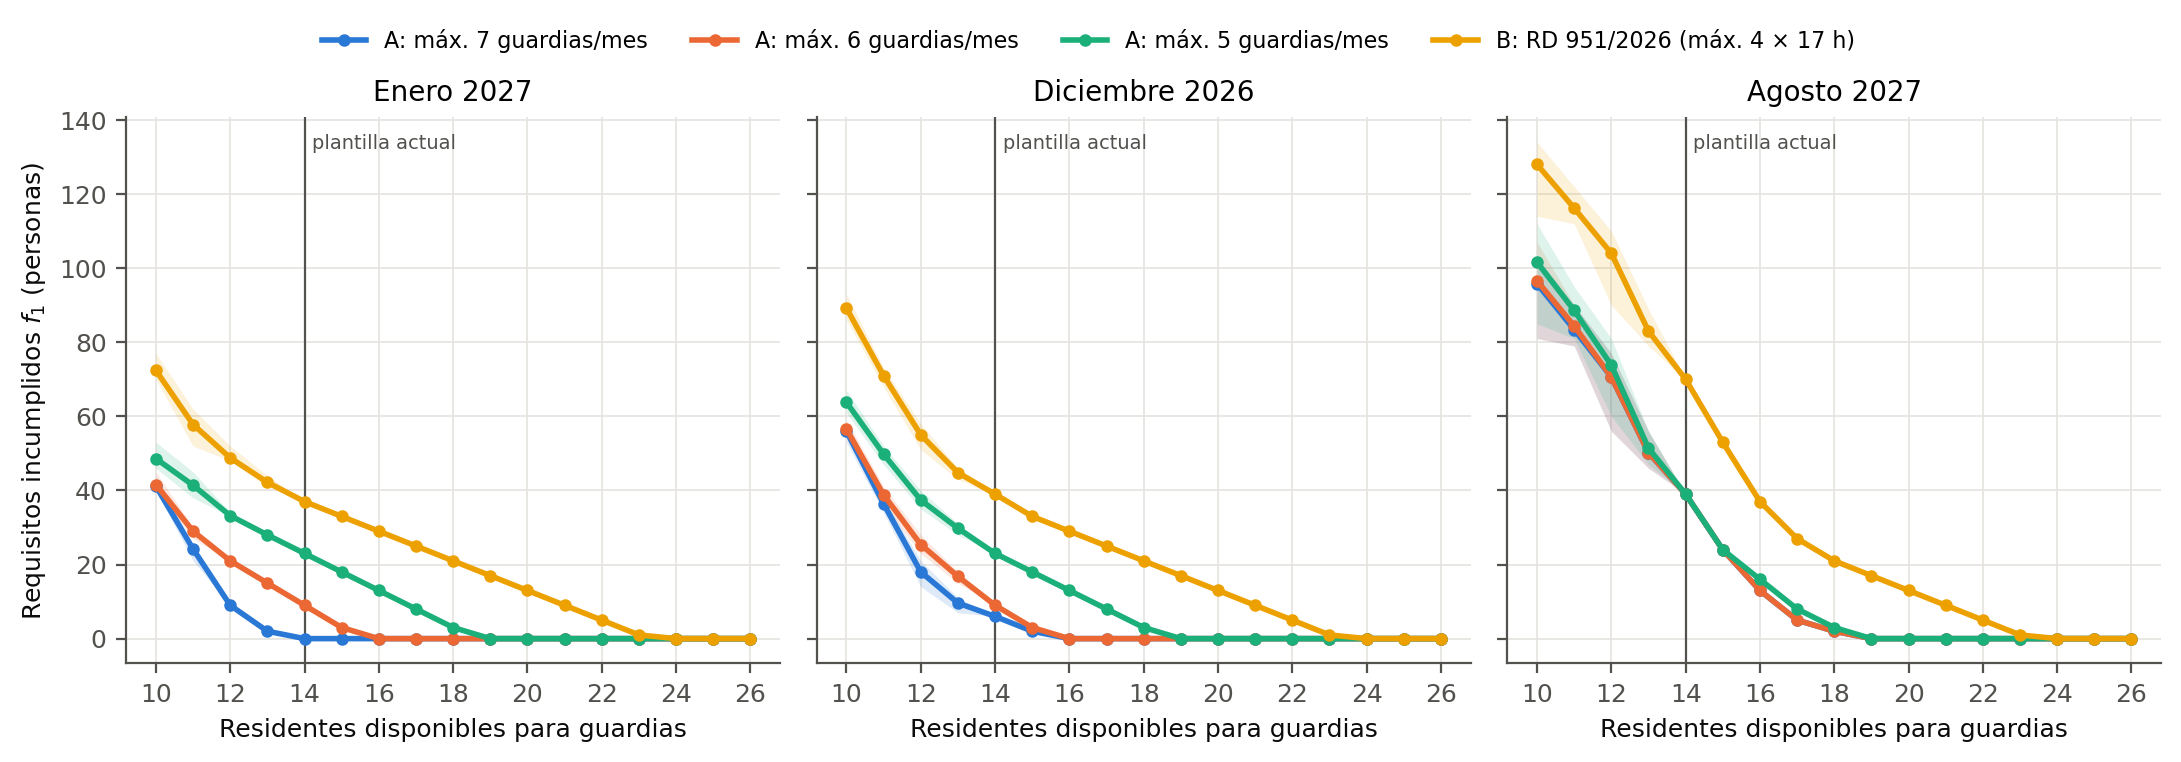
\includegraphics[width=\linewidth]{final_staffing_vs_regime.png}
\caption{Requisitos incumplidos $f_1$ (plazas de guardia, mayores y residentes en planta que faltan) según el número de residentes disponibles para guardias y el límite mensual. A la izquierda de la línea vertical se quitan residentes (media de cinco sorteos; la banda indica el mínimo y el máximo); a la derecha se añaden residentes totalmente disponibles.}
\label{fig:plantilla}
\end{figure}

\begin{table}[ht]
\centering\small
\caption{Residentes disponibles para guardias necesarios para cumplir todos los requisitos ($f_1 = 0$) y, entre paréntesis, para cubrir todas las guardias si se permite reducir la actividad ordinaria. Cota aritmética: $\lceil 93 / \text{máximo mensual} \rceil$. Hoy hay 14.}
\label{tab:plantilla}
\begin{tabular}{@{}lcccc@{}}
\toprule
Régimen & Cota aritmética & Enero 2027 & Diciembre 2026 & Agosto 2027 \\
\midrule
A: máximo 7 guardias (actual)  & 14 & \textbf{14} (14) & \textbf{16} (14) & \textbf{19} (14) \\
A: máximo 6 guardias           & 16 & 16 (16) & 16 (16) & 19 (16) \\
A: máximo 5 guardias           & 19 & 19 (19) & 19 (19) & 19 (19) \\
B: RD 951/2026 (4 de 17 h)     & 24 & \textbf{24} (24) & \textbf{24} (24) & \textbf{24} (24) \\
\bottomrule
\end{tabular}
\end{table}

\paragraph{Lo que recomienda el modelo.}
\begin{itemize}
  \item \textbf{Hoy el servicio no tiene margen.} En enero bastan los 14 residentes disponibles, pero con uno menos ya quedan 2 plazas sin cubrir y todos tienen que hacer el máximo de 7 guardias. El déficit crece cada vez más deprisa: 9 requisitos con dos residentes menos y 41 con cuatro menos, porque a partir de tres ausencias empieza a faltar también personal en planta.
  \item \textbf{El RD 951/2026 exige unos 10 residentes más} (de 14 a 24, un 71\,\% más) para mantener la estructura de guardias actual. En B el cuello de botella es puramente aritmético: cada residente aporta como mucho 4 guardias, cada residente añadido reduce el déficit exactamente en 4 plazas y el modelo alcanza la cota $\lceil 93/4 \rceil = 24$ en los tres meses. La alternativa a contratar es rediseñar las guardias (menos plazas de residente, más adjuntos), y el modelo permite evaluar cada propuesta en segundos.
  \item \textbf{En los meses difíciles el problema no es aritmético.} En diciembre y agosto la cota aritmética del régimen actual (14) no basta: hacen falta 16 y 19 residentes para cumplirlo todo, porque las vacaciones coinciden en los mismos días y cada guardia deja un saliente. Este es el tipo de respuesta que no se obtiene con una hoja de cálculo. Sin embargo, si el servicio acepta reducir la actividad ordinaria, en ambos meses \emph{se pueden cubrir todas las guardias con la plantilla actual} (cifras entre paréntesis): la decisión es de gestión y se analiza en la Sección~\ref{sec:planta}.
  \item \textbf{Un acuerdo local de 5 guardias} costaría tanto como agosto en cualquier mes (19 residentes): las restricciones de calendario dejan de importar porque domina el límite mensual.
\end{itemize}

\subsection{¿Importa quién falta?}

Quitamos dos residentes del mismo año de residencia, probando todas las parejas posibles. En enero el resultado no depende del año: cualquier pareja deja exactamente 9 plazas sin cubrir, que es la diferencia entre las 93 plazas y las $12 \times 7 = 84$ guardias que pueden hacer los 12 restantes. En agosto el déficit varía entre 56 y 77, pero tampoco lo explica el año de residencia, sino la disponibilidad: perder a dos residentes que ya tenían vacaciones cuesta 56--58 requisitos; perder a uno que estaba disponible todo el mes, 66--67, y perder a dos, 77. Con 9 mayores de 15 la exigencia de un mayor por guardia nunca es el problema. \textbf{El recurso escaso son los días-residente disponibles}, así que repartir las vacaciones a lo largo del verano importa más que quién las coge.

\subsection{Guardias frente a actividad ordinaria: el coste de los salientes}
\label{sec:planta}

El objetivo $f_1$ suma con el mismo peso una plaza de guardia sin cubrir y un residente que falta en planta. Por la restricción (9), cada guardia de domingo a jueves deja un saliente que no trabaja al día siguiente. Cuando la planta va justa, cubrir una guardia más cuesta exactamente un residente menos en planta, y el modelo es indiferente entre ambas opciones. Lo comprobamos con una variante que cubre primero las guardias y después la planta (dos niveles lexicográficos en lugar de uno).

\begin{figure}[ht]
\centering
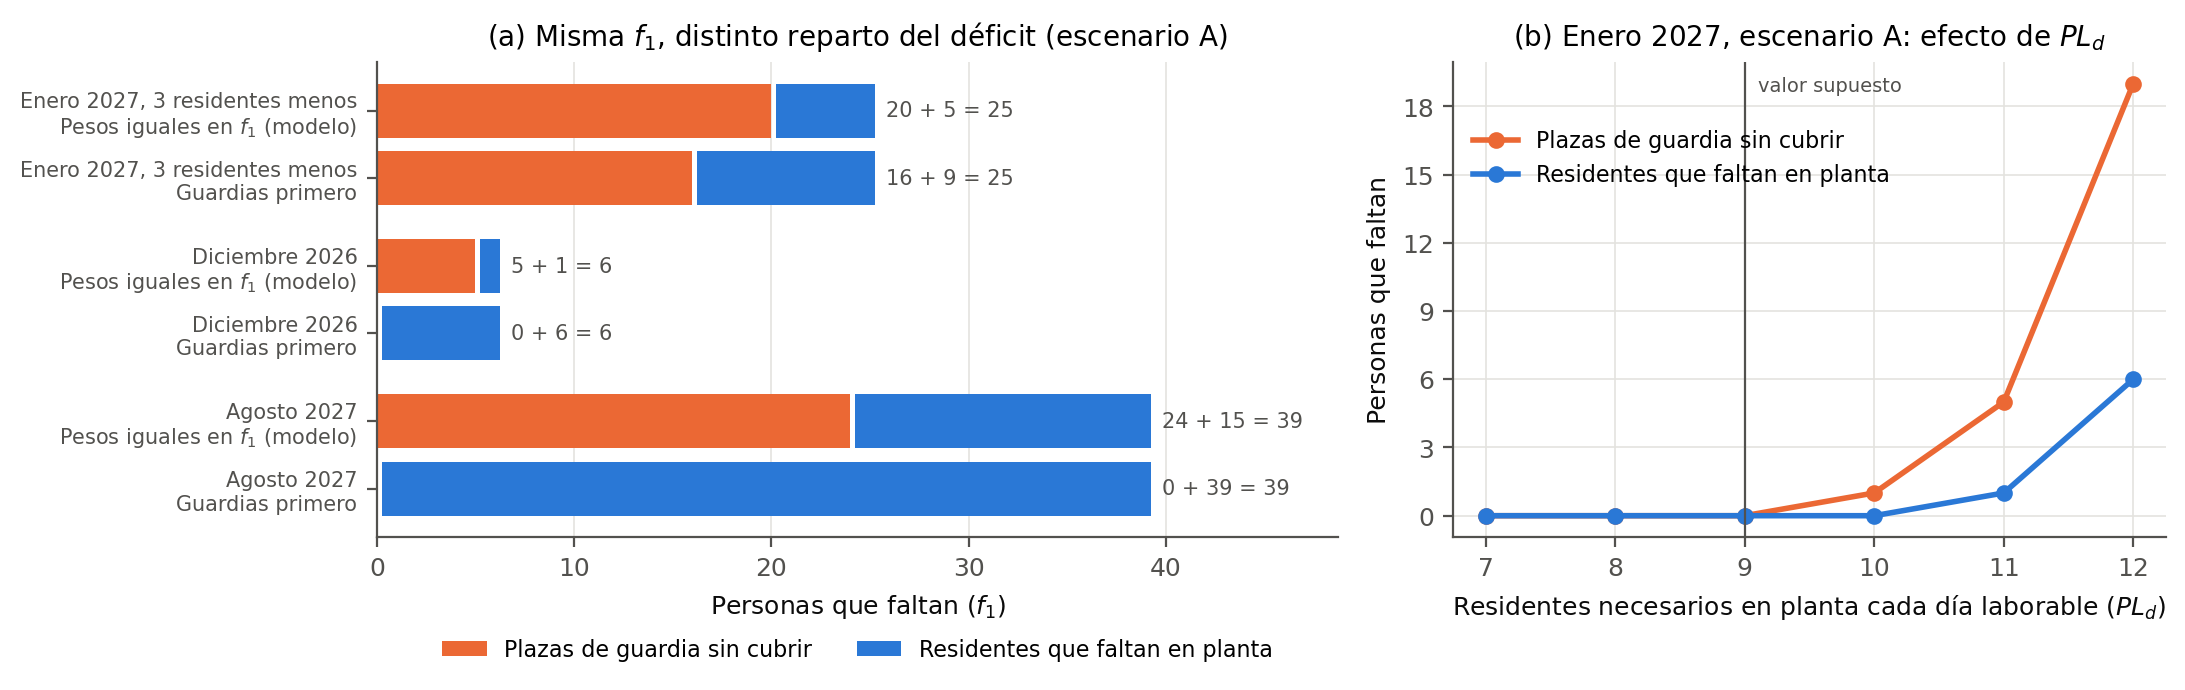
\includegraphics[width=\linewidth]{final_duties_vs_ordinary.png}
\caption{(a) Reparto del déficit $f_1$ entre guardias sin cubrir y residentes que faltan en planta, con el modelo (pesos iguales) y cubriendo primero las guardias. (b) Efecto del número de residentes necesarios en planta cada día laborable ($PL_d$) en enero de 2027, escenario A.}
\label{fig:planta}
\end{figure}

\begin{itemize}
  \item \textbf{El déficit total no cambia, cambia dónde cae} (Figura~\ref{fig:planta}a). En diciembre pasamos de 5 guardias sin cubrir y 1 residente menos en planta a 0 guardias sin cubrir y 6 residentes menos en planta; en agosto, de $24 + 15$ a $0 + 39$. Cada guardia cubierta cuesta un residente-día en planta: el intercambio es 1 a 1.
  \item \textbf{Con la plantilla actual, agosto se puede cubrir} si el servicio acepta tener de media 1,8 residentes menos en planta cada día laborable (39 residentes-día en 22 días laborables). El precio es también el cansancio: cubrir todas las guardias obliga a 16 patrones «día sí, día no» frente a ninguno.
  \item \textbf{Cuando el límite es la capacidad de guardias}, priorizar las guardias ayuda poco: con 3 residentes menos en enero las plazas sin cubrir solo bajan de 20 a 16, que es $93 - 11 \times 7$, el mínimo posible.
  \item \textbf{El requisito de planta supuesto ($PL_d = 9$) está justo en el límite} (Figura~\ref{fig:planta}b). Con $PL_d \le 9$ guardias y planta no compiten en enero; con 10 queda 1 guardia sin cubrir, con 11 quedan 5 guardias y 1 residente en planta, y con 12 el déficit sube a 25. Es uno de los parámetros que más conviene validar con el servicio.
\end{itemize}

\textbf{Implicación.} Que una guardia sin cubrir y un residente menos en planta pesen igual no es una verdad técnica sino una decisión de gestión. Si la urgencia no puede quedar descubierta, el servicio debe usar la variante «guardias primero» y planificar en verano una actividad ordinaria reducida; el modelo dice exactamente cuánta.

\subsection{Equidad a lo largo de varios meses}
\label{sec:equidad}

En un solo mes la equidad mejora poco (Sección~\ref{sec:resultados}). Para ver el efecto a medio plazo, simulamos cinco meses seguidos (enero a mayo de 2027): tras cada mes, el histórico $H_r$, la disponibilidad $\Phi_r$ y las guardias de los dos últimos días ($Y_{rd}$) se actualizan con el cuadrante que acaba de producir el modelo. Comparamos cuatro políticas, evaluadas siempre con la carga acumulada real de cada residente:
\begin{enumerate}
  \item \textbf{Rango con memoria} (el modelo de la Sección~\ref{sec:modelo}).
  \item \textbf{Desviación media con memoria}: $f_3$ se sustituye por la desviación absoluta media de las cargas normalizadas respecto a su media, una métrica alternativa que tiene en cuenta a todos los residentes y no solo a los extremos.
  \item \textbf{Rango sin memoria}: cada mes se equilibra por separado ($H_r = 0$), como haría quien reparte bien los festivos de cada mes sin mirar los anteriores.
  \item \textbf{Sin criterio de equidad}: $f_3$ eliminado.
\end{enumerate}

\begin{figure}[ht]
\centering
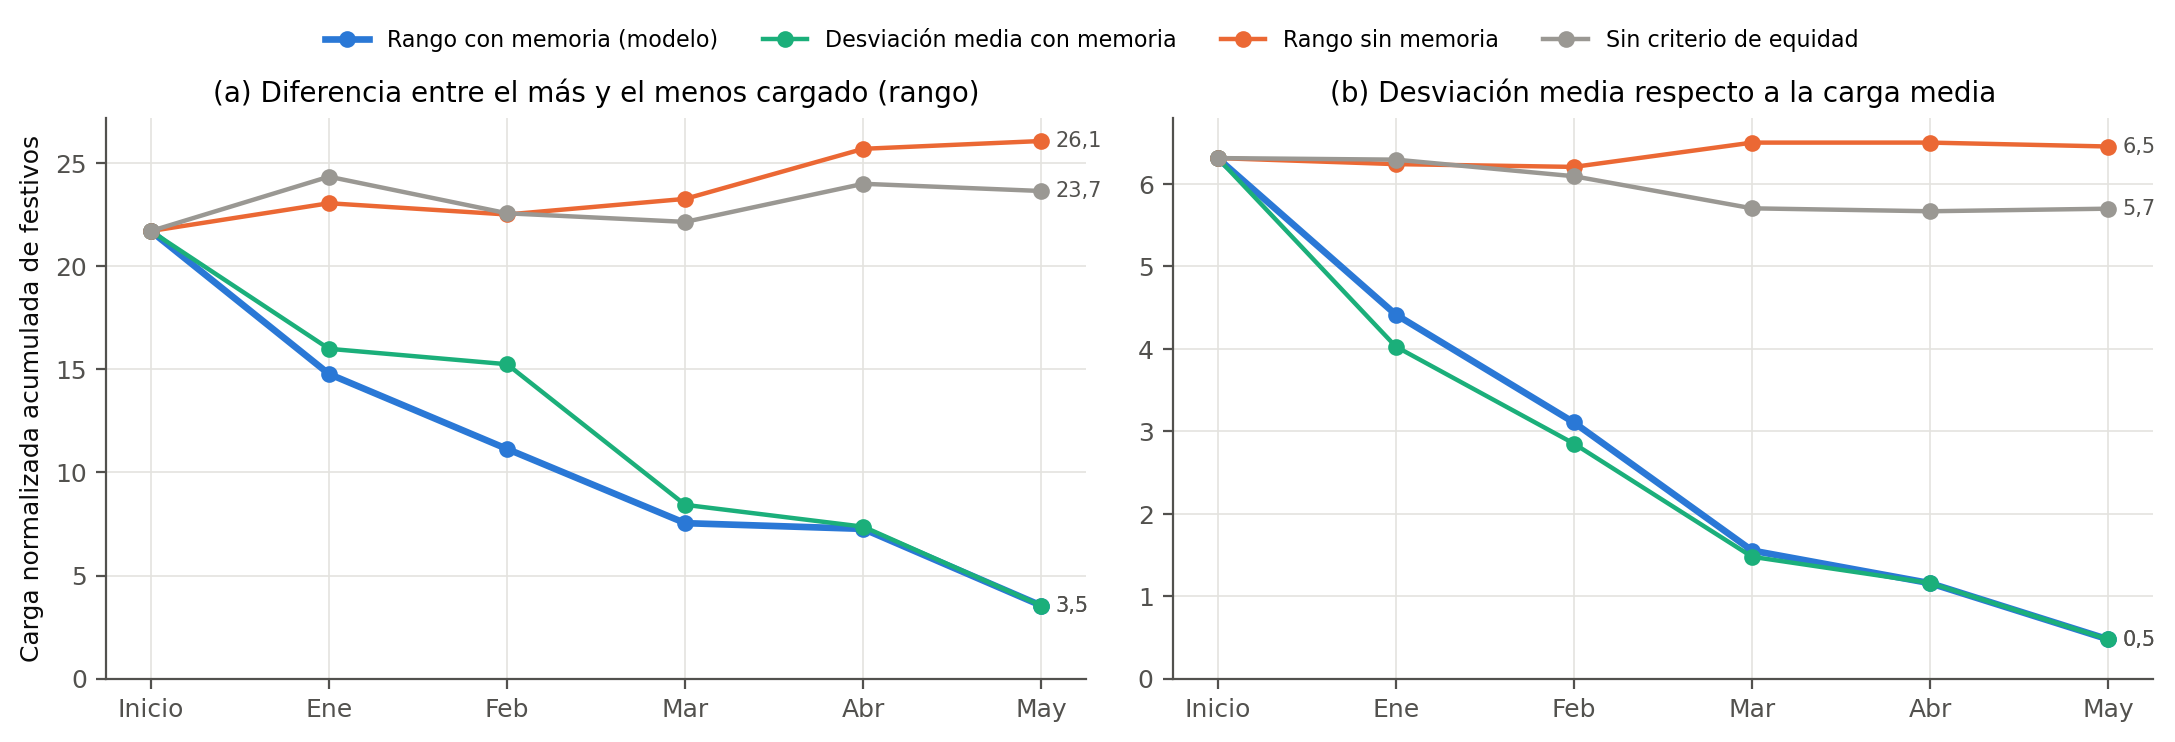
\includegraphics[width=\linewidth]{final_fairness_rolling.png}
\caption{Desigualdad en la carga acumulada de guardias en fin de semana o festivo (normalizada por disponibilidad) a lo largo de cinco meses: (a) diferencia entre el residente más cargado y el menos cargado; (b) desviación absoluta media respecto a la carga media.}
\label{fig:rolling}
\end{figure}

% Numbers from results/tables/final_fairness_rolling.csv (notebook 03, Section 3.4).
\begin{itemize}
  \item \textbf{Con memoria, la desigualdad se reduce mes a mes} (Figura~\ref{fig:rolling}). Con el modelo, la diferencia entre el más y el menos cargado pasa de 21,7 al principio a 14,8 tras enero y a 3,5 tras mayo, y la desviación media baja de 6,3 a 0,5. No cuesta nada: en los cinco meses se cubren todas las guardias ($f_1 = 0$) y se respetan todas las peticiones ($f_2 = 0$).
  \item \textbf{Sin memoria no se corrige nada.} Equilibrar cada mes por separado deja la desigualdad acumulada igual o peor que no tener ningún criterio de equidad: tras mayo el rango es 26,1 sin memoria y 23,7 sin criterio, frente a 3,5 con memoria. Repartir bien los festivos de cada mes da los mismos festivos a quien ya arrastraba un exceso que a quien iba por detrás: \emph{la memoria es lo que hace justo el reparto}.
  \item \textbf{La métrica importa poco a medio plazo.} La desviación media reparte mejor entre los residentes intermedios al principio (4,0 frente a 4,4 tras enero) y el rango protege mejor al más cargado (14,8 frente a 16,0), pero tras cinco meses ambas llegan al mismo reparto (rango 3,5). Recomendamos mantener el rango: es más fácil de explicar («la diferencia entre quien más y quien menos festivos lleva») y se resuelve en menos de un segundo, mientras que la desviación media tarda hasta 36~s en algunos meses.
  \item \textbf{El rango de un solo mes engaña.} En enero el rango se queda en 14,8 aunque cambie la plantilla (Sección~\ref{sec:plantilla}), porque lo fija el residente con más histórico. Visto a lo largo de varios meses el criterio sí funciona: lo que no se puede compensar en un mes se compensa en los siguientes.
\end{itemize}

{\small Detalle técnico: para esta simulación los niveles del objetivo se resuelven uno a uno, con 20~s cada uno. La política sin memoria agota ese límite en el nivel de equidad (tiene muchas soluciones simétricas); las demás se resuelven hasta optimalidad probada.\par}


\subsection{¿Qué aporta cada objetivo?}
\label{sec:objetivos}

Quitamos cada objetivo de menor prioridad por turnos y comparamos el orden lexicográfico con la suma ponderada $1000 f_1 + 100 f_2 + 10 f_3 + f_4$ (Tabla~\ref{tab:objetivos}).

\begin{table}[ht]
\centering\small
\caption{Qué aporta cada objetivo (escenario A). Cada fila elimina un objetivo de menor prioridad o sustituye el orden lexicográfico por la suma ponderada $1000 f_1 + 100 f_2 + 10 f_3 + f_4$.}
\label{tab:objetivos}
\begin{tabular}{@{}llccccc@{}}
\toprule
Mes & Variante & \makecell{$f_1$ (guardias sin\\ cubrir + planta)} & \makecell{Peticiones\\ incumplidas} & \makecell{Rango de\\ festivos $f_3$} & \makecell{Patrones\\ $f_4$} & \makecell{Tiempo\\ (s)} \\
\midrule
\multirow{5}{*}{Enero 2027} & Modelo (lexicográfico) & 0 (0 + 0) & 0/17 & 14{,}8 & 1 & 0{,}3 \\
 & Sin $f_2$ (peticiones) & 0 (0 + 0) & 4/17 & 14{,}8 & 1 & 0{,}3 \\
 & Sin $f_3$ (equidad) & 0 (0 + 0) & 0/17 & 24{,}4 & 0 & 0{,}2 \\
 & Sin $f_4$ (día sí, día no) & 0 (0 + 0) & 0/17 & 14{,}8 & 16 & 0{,}2 \\
 & Suma ponderada & 0 (0 + 0) & 0/17 & 14{,}9 & 0 & 0{,}2 \\
\midrule
\multirow{5}{*}{Diciembre 2026} & Modelo (lexicográfico) & 6 (5 + 1) & 0/12 & 23{,}1 & 0 & 0{,}3 \\
 & Sin $f_2$ (peticiones) & 6 (5 + 1) & 4/12 & 23{,}1 & 0 & 0{,}2 \\
 & Sin $f_3$ (equidad) & 6 (6 + 0) & 0/12 & 29{,}0 & 0 & 0{,}2 \\
 & Sin $f_4$ (día sí, día no) & 6 (6 + 0) & 0/12 & 23{,}1 & 23 & 0{,}2 \\
 & Suma ponderada & 6 (5 + 1) & 0/12 & 23{,}1 & 0 & 0{,}1 \\
\midrule
\multirow{5}{*}{Agosto 2027} & Modelo (lexicográfico) & 39 (24 + 15) & 0/21 & 9{,}8 & 0 & 0{,}2 \\
 & Sin $f_2$ (peticiones) & 39 (21 + 18) & 4/21 & 5{,}5 & 1 & 0{,}2 \\
 & Sin $f_3$ (equidad) & 39 (24 + 15) & 0/21 & 13{,}2 & 0 & 0{,}2 \\
 & Sin $f_4$ (día sí, día no) & 39 (22 + 17) & 0/21 & 9{,}8 & 14 & 0{,}2 \\
 & Suma ponderada & 39 (21 + 18) & 0/21 & 9{,}8 & 0 & 0{,}1 \\
\bottomrule
\end{tabular}
\end{table}


\begin{itemize}
  \item \textbf{Las peticiones y los patrones salen gratis en cobertura.} Sin $f_2$ el modelo incumple 4 peticiones en cada mes sin reducir en nada los requisitos incumplidos $f_1$; sin $f_4$ aparecen 16, 23 y 14 patrones «día sí, día no» donde el modelo deja 1, 0 y 0. Los dos objetivos cambian mucho la calidad del cuadrante para los residentes sin coste para el servicio.
  \item \textbf{En agosto, peticiones y equidad compiten.} Si se ignoran las peticiones, el rango de festivos baja de 9,8 a 5,5 a cambio de incumplir 4 de 21 peticiones. El orden de prioridades (peticiones antes que equidad) es una decisión que el servicio debe tomar conscientemente; el modelo cuantifica su precio.
  \item \textbf{Sin criterio de equidad} el rango acumulado de festivos empeora incluso respecto al de partida en enero (de 21,7 a 24,4) y en diciembre (de 27,5 a 29,0).
  \item \textbf{La suma ponderada no respeta las prioridades.} En enero cambia equidad por patrones (rango 14,9 en lugar de 14,8, a cambio de quitar un patrón, porque $10 \times 0{,}08 < 1$). En agosto alcanza el mismo $f_1 = 39$ pero lo reparte de otra forma ($21 + 18$ en lugar de $24 + 15$): entre soluciones empatadas elige de forma arbitraria. El orden lexicográfico evita tener que calibrar pesos y se resuelve igual de rápido.
\end{itemize}

\subsection{Validez y limitaciones del análisis}

\begin{itemize}
  \item \textbf{Datos sintéticos.} Las cifras dependen de los supuestos de la Tabla~\ref{tab:supuestos}. Los mecanismos (el coste de los salientes, el límite aritmético en B, el efecto de la memoria) son robustos; las cifras exactas deben recalcularse con los datos del servicio. Los parámetros más influyentes son $PL_d$, los límites mensuales y la estructura de guardias.
  \item \textbf{Escenario B aproximado.} Suponer que todas las guardias son de 17~h ignora que las de 24~h de fin de semana tendrán que partirse en dos módulos, lo que probablemente aumentará las necesidades. Tampoco modelamos el descanso semanal de 24~h ni la media de 45~h semanales del RD 951/2026, porque no modelamos el horario de la jornada ordinaria.
  \item \textbf{Residentes añadidos optimistas.} Los residentes sintéticos añadidos están disponibles todo el mes; uno real también tendría vacaciones, así que las cifras de la Tabla~\ref{tab:plantilla} para agosto son una cota inferior.
  \item \textbf{Varios cuadrantes óptimos.} Los valores de $f_1$ a $f_4$ son únicos, pero puede haber varios cuadrantes que los alcancen. Indicadores que no se optimizan (como el reparto de guardias por residente) pueden cambiar entre ejecuciones o versiones del solver; si el servicio los considera importantes, deberían convertirse en objetivos.
\end{itemize}

% =====================================================================
\section{Conclusiones y recomendaciones}
\label{sec:conclusiones}

Hemos formulado el cuadrante mensual de guardias de residentes como un modelo de programación entera con cuatro objetivos jerarquizados que \emph{siempre} devuelve un cuadrante: si el mes no se puede cubrir, dice exactamente qué falta y cuándo. El modelo se resuelve en menos de un segundo y cada cuadrante se valida de forma independiente. Respondiendo a las preguntas del inicio:

\begin{enumerate}[label=\textbf{P\arabic*.}]
  \item \textbf{Cobertura.} En un mes normal la plantilla actual lo cubre todo, respeta todas las peticiones y casi no genera patrones agotadores, pero sin ningún margen. En diciembre y agosto quedan huecos (6 y 39 requisitos) que el modelo localiza día a día.
  \item \textbf{Plantilla.} Con el RD 951/2026 y la estructura de guardias actual el servicio necesita unos 24 residentes disponibles en lugar de 14. En el régimen actual necesita 16 en Navidad y 19 en agosto para cumplir también con la actividad ordinaria, o puede cubrir todas las guardias con los 14 actuales reduciendo la actividad ordinaria.
  \item \textbf{Equidad.} Equilibrar cada mes por separado no corrige un reparto heredado injusto; con memoria, la desigualdad acumulada se reduce mes a mes.
  \item \textbf{Prioridades.} Respetar las peticiones y evitar los patrones «día sí, día no» no cuesta cobertura. Las decisiones con un precio real son dos: guardias frente a actividad ordinaria y, en meses tensos, peticiones frente a equidad.
\end{enumerate}

\paragraph{Recomendaciones para el servicio.}
\begin{enumerate}
  \item \textbf{Usar el modelo cada mes} en lugar del cuadrante manual: da un cuadrante óptimo y auditable en segundos y señala los huecos con antelación.
  \item \textbf{Preparar ya la transición a septiembre de 2027.} Con la estructura actual harían falta unos 10 residentes más. El servicio debería decidir entre ampliar la plantilla y rediseñar las guardias (menos plazas cubiertas por residentes, módulos más cortos o más adjuntos) y usar el modelo para comparar las propuestas.
  \item \textbf{Decidir explícitamente qué va primero en verano}: la urgencia o la actividad ordinaria. Si es la urgencia, programar en agosto una actividad ordinaria reducida (unos 2 residentes menos al día) y escalonar las vacaciones para que no coincidan.
  \item \textbf{Mantener la equidad con memoria a lo largo del año de residencia}, que es lo que corrige los desequilibrios heredados.
  \item \textbf{Validar con el servicio los parámetros más influyentes}: residentes necesarios en planta, límites mensuales, quién cuenta como mayor y la nueva estructura de guardias.
\end{enumerate}

\paragraph{Trabajo futuro.} (i) Validar los supuestos y recalcular los resultados con datos reales del hospital. (ii) Modelar el escenario B con los nuevos tipos de guardia y su duración $T_g$ (restricción 10 completa). (iii) Reprogramar ante ausencias imprevistas con el mínimo número de cambios, $\min \sum |x_{rdg} - \hat x_{rdg}|$, y evaluar la robustez del cuadrante con simulación Monte Carlo de bajas.

% =====================================================================
\clearpage
\appendix
\section{Cambios respecto a la propuesta}
\label{app:feedback}

La Tabla~\ref{tab:cambios} resume cómo hemos incorporado los comentarios a la propuesta del 11 de octubre y qué otros cambios de modelado hemos hecho desde entonces.

{\small
\begin{longtable}{@{}p{2.8cm}p{3.5cm}p{4.2cm}p{4.6cm}@{}}
\caption{Cambios en la formulación desde la propuesta.}\label{tab:cambios}\\
\toprule
Elemento & Propuesta & Ahora & Motivo \\
\midrule
\endfirsthead
\toprule
Elemento & Propuesta & Ahora & Motivo \\
\midrule
\endhead
Notación & Mayúsculas y minúsculas mezcladas ($e_{rdg}$, $E^{\max}$) & Parámetros en mayúsculas ($E_{rdg}$, $ROT_{rd}$, $PL_d$); variables en minúsculas ($e^{\max}$, $e^{\min}$) & Comentario del profesor \\
Descripción de los parámetros & Etiquetas breves & Significado de cada subíndice (p.\,ej., $N_{dg}$: residentes necesarios para cubrir la guardia de tipo $g$ el día $d$) & Comentario del profesor \\
Restricción (7) & $y_{rd} \le s_{rd}$ y se penaliza $s_{rd}$ & Sin restricción: $f_2$ penaliza directamente $Q_{rd}\,y_{rd}$ & El profesor no veía la conexión; $s_{rd} = y_{rd}$ en todo óptimo, así que era redundante \\
Restricción (9) & Una versión y una nota & Explicación detallada de los salientes y una versión por escenario normativo & Comentario del profesor; el RD 951/2026 limita jornada más guardia consecutivas a 17~h \\
Prioridad de las peticiones & $w_{rd}$ & $Q_{rd}$ & Evitar confusión con los pesos $W^k$ \\
Restricciones (2), (6) y (9) & Duras & Con variables de déficit penalizadas en $f_1$ & Las versiones duras podían hacer el modelo infactible, contra el objetivo de decir qué guardias quedan sin cubrir \\
Equidad (8) & $\Phi_r$ = fracción del año; todos los residentes & $H_r$ y $\Phi_r$ referidos al mismo periodo; solo $\mathcal{R}^F$ & El numerador y el denominador deben referirse al mismo periodo; quien no puede recibir festivos fijaría $e^{\max}$ o $e^{\min}$ \\
Restricción (5) & Enlazada con el día 0 & Enlazada con los días $-1$ y $0$ & Detectar el patrón al cambiar de mes \\
Objetivo & Suma ponderada con $W^1 \gg W^2 \gg W^3 \gg W^4$ & Lexicográfico (jerárquico de Gurobi) & Prioridades exactas sin problemas numéricos (Sección~\ref{sec:objetivos}) \\
Escenario 2027 & Proyecto de real decreto; $c_r \le \kappa_r$ como decisión & RD 951/2026 aprobado; $C_r$ como dato & El módulo adicional solo cabe por razones formativas y con consentimiento \\
\bottomrule
\end{longtable}
}

\section{Contenido de la entrega y reproducción}
\label{app:entrega}

\begin{center}\small
\begin{tabularx}{\linewidth}{@{}lX@{}}
\toprule
Ruta & Contenido \\
\midrule
\texttt{informe\_final.pdf} & Este informe. \\
\texttt{README.md} & Instrucciones de instalación y ejecución. \\
\texttt{requirements.txt} & Dependencias de Python. \\
\texttt{notebooks/01\_synthetic\_data\_generation.ipynb} & Generador de datos sintéticos (Sección~\ref{sec:datos}). \\
\texttt{notebooks/02\_baseline\_model.ipynb} & Modelo, resolución, validación e indicadores (Secciones~\ref{sec:modelo} y \ref{sec:impl}). \\
\texttt{notebooks/03\_analysis.ipynb} & Resultados y análisis de sensibilidad (Secciones~\ref{sec:resultados} y \ref{sec:analisis}). \\
\texttt{data/synthetic/} & Las siete instancias (CSV y \texttt{meta.json} con la configuración y la semilla). \\
\texttt{results/tables/}, \texttt{results/figures/} & Tablas y figuras generadas por los notebooks (prefijo \texttt{final\_} para las de este informe). \\
\texttt{report/} & Código fuente \LaTeX{} de este informe. \\
\bottomrule
\end{tabularx}
\end{center}

Para reproducir los resultados: \texttt{pip install -r requirements.txt}, instalar una licencia académica de Gurobi y ejecutar los tres notebooks en orden desde la carpeta \texttt{notebooks/}. El notebook 03 tarda unos 11 minutos.


\end{document}
